\documentclass[letterpaper,twocolumn,10pt]{article}
\usepackage{epsfig,endnotes}
\usepackage{times}
\usepackage{url}
\usepackage{graphicx}
\usepackage{subfigure}
\usepackage{balance}  % for  \balance command ON LAST PAGE  (only there!)
\usepackage{algpseudocode,algorithm}
\usepackage{epstopdf}
\usepackage{comment}
\usepackage{color}
\usepackage{multirow}
\usepackage[normalem]{ulem}
% do not change these values
% TEMPLATE for Usenix papers, specifically to meet requirements of
%  USENIX '05
% originally a template for producing IEEE-format articles using LaTeX.
%   written by Matthew Ward, CS Department, Worcester Polytechnic Institute.
% adapted by David Beazley for his excellent SWIG paper in Proceedings,
%   Tcl 96
% turned into a smartass generic template by De Clarke, with thanks to
%   both the above pioneers
% use at your own risk.  Complaints to /dev/null.
% make it two column with no page numbering, default is 10 point

% Munged by Fred Douglis <douglis@research.att.com> 10/97 to separate
% the .sty file from the LaTeX source template, so that people can
% more easily include the .sty file into an existing document.  Also
% changed to more closely follow the style guidelines as represented
% by the Word sample file.

% Note that since 2010, USENIX does not require endnotes. If you want
% foot of page notes, don't include the endnotes package in the
% usepackage command, below.

% This version uses the latex2e styles, not the very ancient 2.09 stuff.

\begin{document}

%don't want date printed
\date{}

%make title bold and 14 pt font (Latex default is non-bold, 16 pt)
\title{\Large \bf EARNCache: Self-adaptive Incremental Big Data Caching on Non-Big Clusters}

%for single author (just remove % characters)
\author{
{\rm Junshi Guo}\\
Fudan University
\and
{\rm Yifeng Luo}\\
Fudan University
\and
{\rm Eric Lo}\\
The Chinese University of Hong Kong
\and
{\rm Shuigeng Zhou}\\
Fudan University
} % end author
% copy the following lines to add more authors
% \and
% {\rm Name}\\
%Name Institution

\maketitle

% Use the following at camera-ready time to suppress page numbers.
% Comment it out when you first submit the paper for review.
\thispagestyle{empty}


\subsection*{Abstract}
Memory caching plays a crucial role in determining whether people's requirements on (quasi-)real-time processing of exploding data on big-data clusters could be satisfied. As big data clusters usually are concurrently shared by multiple computing frames, applications or end users, there exists intense competition for memory cache resources, especially on small clusters which are supposed to process big datasets comparable to large clusters \textcolor{red}{yet} with tightly limited resources. Applying existing on-demand caching strategies on small shared clusters inevitably results in frequent cache thrashings when the conflicts of simultaneous cache resource demands are not mediated, and then the running efficiency of the whole big data cluster will be deteriorated.

In this paper, we propose a novel self-adaptive incremental big data caching mechanism, called \textcolor{red}{EARNCache}, to improve the cache efficiency for shared big data clusters, especially for small clusters where cache thrashings are more likely to occur. \textcolor{red}{EARNCache} self-adaptively adjusts resource allocation strategies according to the competition condition of cache resources: evolving to incremental caching to depress competition when resources are in deficit, devolving to traditional on-demand-caching to expedite data caching-in when resources are in surplus. Our experimental evaluation shows that \textcolor{red}{EARNCache}'s elasticity could enhance the cache efficiency for shared big data clusters, with improved resource utilization.

\section{Introduction}\label{sec:Introduction}

The Internet has enabled and popularized DBaaS~\cite{PDBaaS,RMTD,salesforce,Force,MTDB1,DBMaaS,DBaaS}, where service providers host database applications on their infrastructures, and deliver them as services to different end users ~(also called tenants), who would otherwise need to deploy these database applications by themselves. Tenants who have subscribed DBaaS services could query and update their data via web browsers or client programs, so the ownership and operation of database applications are outsourced to DBaaS service providers. DBaaS service providers typically consolidate multiple tenants into the same hardware/software platform so as to reduce operational cost via resource sharing.

When tenants necessitate QoS guarantees and require satisfaction of performance SLOs, service providers usually have to reserve resources for tenants according to their performance SLOs, so that a database server would always have enough processing capacity to handle all tenants' workloads consolidated on this server, under various workload conditions. However, service providers could only achieve moderate resource utilizations in such a resource-reservation tenant consolidation fashion. DBaaS tenants often quantify their resource requirement according to the peaks of their workloads, and they usually tend to over-estimate their performance SLOs to make sure that subscribed resources could completely cover the actual resource needs of their businesses, so the workload pressure generated by a tenant will not be persistently intense enough to catch up with this tenant's performance SLO. What's more, multi-tenancy tends to possess low overall tenant activeness, and there exist few chances that massive tenants would generate their workloads at their full speeds concurrently, so the DBaaS system would witness moderate resource utilizations most of the time.

Carlo Curino et al.~\cite{Workload-Aware} proposed a buffer pool gauging procedure, included in their tenant consolidation scheme named Kairos for their multi-tenant database platform~\cite{Relational}, to estimate the working set size of a database workload, so that they could properly accomplish consolidation for multiple database workloads with minimum servers. However, this buffer pool gauging procedure is not applicable for our targeting scenario. The difficulty is twofold: firstly, to precisely quantify a tenant's resource demands requires the tenant's workload to be stable, while it is impossible to accomplish precise quantifications if the tenant's workload changes dynamically over time; secondly, when far more tenants are consolidated into the same database, there is no reliable mechanism for guaranteeing that memory resources are allocated to processing workloads which actually require more resources. As a huge amount of tenants are consolidated into the same database, buffer resources allocated to tenants with high-intensity workloads may be spared for other massive numbers of tenants with low-intensity workloads, and precious memory resources are not persistently employed to buffer data for those tenants with high-intensity workloads but wasted on buffering data for tenants with low-intensity workloads. So our targeting scenario requires an effective mechanism which could dynamically quarantine tenants with high-intensity workloads from tenants with low-intensity workloads, which could guarantee that processing of high-intensity workloads would not affect by low-intensity workloads, and thus the DBaaS system could get the most out of resources allocated to process high-intensity workloads.

Targeting at application scenarios where thousands of small tenants with low overall tenant activeness and yet with various database schemas should be served with QoS guarantees, we propose a novel multi-tenant database system called FrugalDB to further improve resource utilization and reduce operational cost, where small tenants' database sizes are expected to be at tens of or a few hundred megabytes scales and their workloads usually exhibit obvious unstableness with huge variance. FrugalDB could consolidate more tenants with performance SLOs onto the same database server. While for medium or large tenants whose database sizes grow up to gigabytes with strict QoS requirements and stable workloads, we think it would be much more appropriate to adopt the shared-machine scheme, which encapsulates different tenants' database in different properly configured virtual machines~(VMs) running independent databases, and it is out of this paper's discussion scope.

We mainly make the following three contributions in this paper: ~1) propose a workload offloading mechanism to handle mixed workloads of tenants with performance SLOs; ~2) formulate and solve the workload offloading problem as an optimization problem; ~3) implement a prototype of the proposed workload offloading mechanism, and perform extensive experiments to evaluate the efficiency of the mechanism. In the remainder of this paper, we first introduce the system design and implementation details about FrugalDB in Sec.~\ref{sec:SDI}, and formally define the targeting problem and present the algorithms employed to solve the problem in Sec.~\ref{sec:PFA}. We provide experimental results to validate FrugalDB's efficiency in Sec.~\ref{sec:Experiments}, and present the related work of FrugalDB in Sec.~\ref{sec:RelatedWork}. Sec.~\ref{sec:Conclusion} concludes this paper. 

%\section{Motivation}\label{sec:Motiv}

Big data application characteristics Write-Once-Read-Many~(WORM), file scan, all blocks of a file possess almost the same recency and frequency property. This is unlike Web applications or traditional OLTP database applications, where various ranges or blocks of the same dataset may possess far different recency and frequency property.

Unlike traditional operating-system-level or database-level data caching, where caching is executed on small data units (i.e. 8KB-sized pages), big data caching are executed on big data units(i.e. 256MB-sized blocks), so the cost of caching in/out a data unit for big data far exceeds that for traditional data caching. For example, caching in an 8KB-sized page may take milliseconds, while caching in a 256MB-sized block may take seconds. Besides, traditional operating-system-level or database-level data caching may have millions of slots for caching data units, and this makes hotter data units less likely cached out by colder data units; big data caching may only have thousands of slots for caching data units, and thus hotter data units have much higher likelihood of being cached out by colder data units.

When memory cache resources of a big data cluster are shared by multiple computing frames, applications or end users, multiple cache resource demands may be concurrently generated from various computing frames, applications or end users. These concurrent resource demands could leads to serious cache resource conflicts on a non-big cluster with relatively limited cache capacity, compared to the aggregate of concurrent resources demands. Competition for computational resources does not have obviously decrease computation efficiency, while competition for cache resources may obviously decrease cache efficiency, because of data caching in/out cost. If cache resource conflicts occur temporarily, cache efficiency would only be influenced for the time being; while if the resource conflicts endure, cache thrashings would be incurred continuously because of massive and frequent cache block replacements, and the cache efficiency would deteriorate ceaselessly, making the whole cluster gain few benefits from data caching. This is the reason why we need to revisit existing caching mechanisms and strategies, and propose more effective measures to improve the efficiency of data caching on non-big clusters.

Let's take the following example to illustrate the problem of cache resource competition on non-big clusters shared by multiple users. Assume: we have a cluster consisting of 20 nodes; each node could spare 50GB DRAM memory resources for data caching, which means the cluster possesses a 1000GB cache capacity; the cluster is concurrently shared by 8 end users, each of which needs 200GB cache resources for real-time analytical data processing, and all data are uniformly dispersed across the whole cluster; all analytical jobs submitted by different users are run one by one. We illustrate the cache efficiency of various workload constitutions achieved with different caching strategies in Tab.~\ref{Tab:example1}, where $J_{i}$ denotes the analytical job of $User_{i}$, caching strategy denotes the resource allocation strategy and corresponding replacement policy, and the cache efficiency is defined as:
\begin{equation}
cache\_efficiency = \frac{Volume of Data Obtained in Cache}{Total Volume of Data Accessed}
\end{equation}

\begin{table}[!htb]
\caption{Cache efficiency of various workloads with different caching strategies.}
\label{Tab:example1}
\centering
\begin{tabular}{|c|c|c|c|}
\hline
Workload & Caching Strategy & Efficiency\\
\hline
\multirow{3}{*}{{\shortstack{J1,J2,J3,J4,J5,J6,J7,J8 \\ \ldots \ldots}}} & On-Demand/LRU & 0\% \\
\cline{2-3}
&On-Demand/LFU & 0\% \\
\cline{2-3}
& Fair Share & 0\% \\
\hline
\multirow{3}{*}{{\shortstack{J1,J2,J3,J4,J5,J6,J7,J8\\ \ldots \ldots}}} & On-Demand/LRU & 0\% \\
\cline{2-3}
&On-Demand/LFU & 0\% \\
\cline{2-3}
& Fair Share & 0\% \\
\hline
\multirow{3}{*}{{\shortstack{J1,J2,J3,J4,J5,J6,J7,J8\\ \ldots \ldots}}} & On-Demand/LRU & 0\% \\
\cline{2-3}
&On-Demand/LFU & 0\% \\
\cline{2-3}
& Fair Share & 0\% \\
\hline
\end{tabular}
\end{table}




\renewcommand{\algorithmicrequire}{\textbf{Input:}}
\renewcommand{\algorithmicensure}{\textbf{Output:}}

\section{System Framework}\label{sec:SDI}
We mainly illustrate how \textcolor{red}{EARNCache} works in this section. Firstly we present the overview about the cache-earning mechanism of \textcolor{red}{EARNCache}, and then illustrate its architecture design, and finally explains the incremental cache-earning policy and its implementation.

\subsection{Overview}\label{sec:overview}

On shared non-big clusters with relatively limited cache capacity, cache resource conflicts \textcolor{red}{\sout{on non-big clusters}} would be \textcolor{yellow}{norm rather than exception}. When only quite few users are using a non-big cluster and the competition for cache resources is mild, applying on-demand caching could expedite hotter blocks taking over cache resources from colder blocks, and hotter data is less likely to be cached out by colder data. When more concurrent users are using the cluster and the competition for cache resources gets wild, on-demand caching leaves concurrently cache resource demands unmediated, which makes hotter data more vulnerable to being cached out. Files which are frequently accessed recently sometimes could be totally cached out by files which would rarely be accessed for the second time in the near future, then these hot cached-out files need caching in soon as their next access should occur in the incoming future. We consequently need to revisit existing on-demand caching mechanisms and strategies, and propose more effective measures to improve the efficiency of data caching on non-big clusters.

We believe that a good caching strategy for non-big clusters should be self-adaptive to resource competition conditions to depress competitions and avoid thrashings when resources are in desperate deficit. Obviously caching big data files on demand as a whole could not provide such self-adaptivity. Intuitively we should not cache files entirely \textcolor{red}{\sout{when caching them entirely causes tension. }}
Not compulsorily caching files entirely provides the elasticity of tuning the amount of cache resources allocated for different files, according to the files' access recency and frequency.

Ideally, more \textcolor{red}{recently frequently accessed files} should be assigned with more cache resources, \textcolor{red}{and less recently frequently accessed files}
%and less frequently accessed files recently 
should be assigned with less cache resources. However, \textcolor{red}{it's not possible to know in advance what files would be frequently accessed in the upcoming future and we could only make predictions based on historical file access patterns, especially the most recent information.}
%it's impossible to know for sure what files would be frequently accessed files recently, and we could only make predictions based on available historical file access information, especially recent accesses. 
Based on files' historical access information, \textcolor{red}{EARNCache} implements an incremental caching strategy, where a user should earn resources to cache files from other concurrent users via accessing these files. Cache resources are incrementally allocated to files becoming frequently accessed, which gradually takes over cache resources from files getting less frequently accessed, until all blocks of the file have been cached in. The more a \textcolor{red}{file} is accessed, the more cache resources it takes over. The incremental caching strategy ensures that cached hot files being frequently accessed recently will not be flushed out by other massive less hot files, which may only be accessed occasionally or randomly.

\subsection{Architecture}\label{sec:Arch}
Cached files originally are stored in the under distributed file system (i.e. Hadoop File System), and \textcolor{red}{EARNCache} \textcolor{red}{\sout{globally}} coordinately cache them across the whole cluster. \textcolor{red}{EARNCache}'s architecture consists of a central \emph{master} and a set of \emph{workers} residing on storage nodes of the cluster(see Fig.~\ref{fig:Arch}). 
The master's main role is: ~1) to determine how many cache resources should be allocated to a file, based on the resource competitions; ~2) to inform workers of cache resource allocation plans via heartbeats; ~3) to \textcolor{red}{keep} track of cache metadata about which storage node a cached block resides on; ~4) to answer clients' queries on cache metadata. \textcolor{red}{And} the worker's main role is: ~1) to receive resource allocation plans from the master; ~2) to calculate how many resources a file should contribute to compose the allocated resources; ~3) to cache in/out blocks according to the calculated resource composition plans; ~4) to inform the master of cached blocks via heartbeats; ~5) serve clients with cached blocks.

The procedures of a client accessing a block are: ~1) the client queries the master where the block is located; ~2) the master tells the client which worker it should contact to access the block; ~3) the client contacts the worker to access the block; ~4) the worker serves the client with the block data from cache. One thing worth noting here is that: the client will not contact any worker to access a block if the block has been cache out, as the master only keeps track of cached blocks, and could not provide the client with information about \textcolor{red}{cached-out blocks}, then the client has to turn to the under file system for this block.


\begin{figure}[!htbp]
\centering
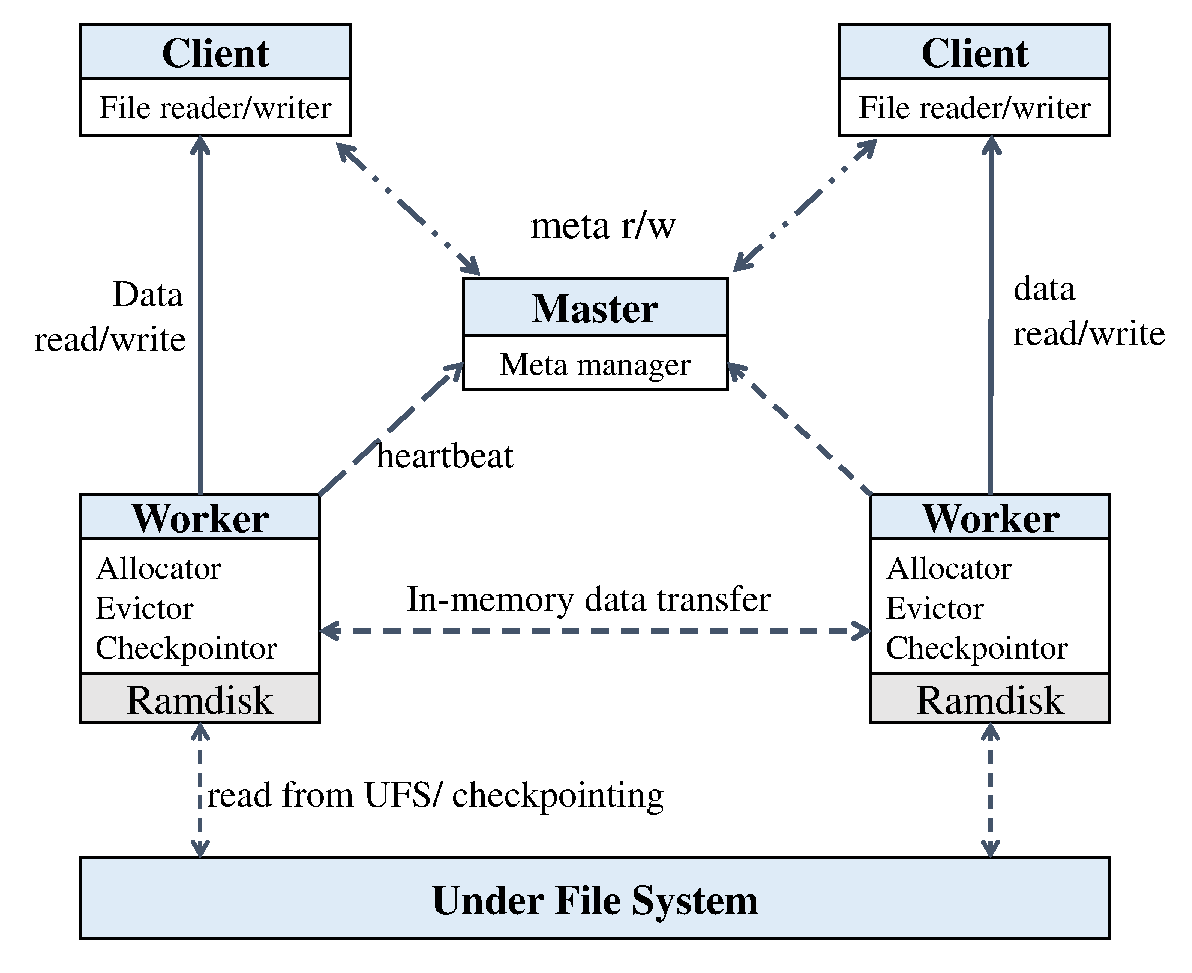
\includegraphics[scale=0.4]{figures/architecture.eps}
\caption{EARNCache's Architecture.}
\label{fig:Arch}
\end{figure}

%Competition for computational resources rarely influences the completion of running tasks, namely each of the scheduled concurrent tasks may run as fast as it runs alone. does not have obviously decrease computation efficiency, as ; while competition for cache resources may seriously decrease cache efficiency, because of data caching in/out cost.
%Big data applications usually access files in a scan fashion and datasets are usually prohibitively huge in size.
%Work about on-demand caching mainly focuses on cache replacement policies, and most replacement policies are variants of LRU, LFU or LRU-LFU-combined.

\subsection{Incremental Caching}\label{sec:framework master}

As we prefer to letting frequently accessed files recently incrementally take over resources from less frequently accessed files recently, "recently" should be defined quantitatively before we could design the incremental caching strategy, and other related elements should also be defined. Tab.~\ref{tab:notation} presents all definitions of notations involved in our incremental caching strategy.
\begin{table}[!htb]
	\caption{Notation definitions}
	\label{tab:notation}
	\centering
	\begin{tabular}{|p{0.15\linewidth}|p{0.75\linewidth}|}
		\hline
		Notation & Definition\\
		\hline
		$W$ & predefined window size of the most recently accessed data for observing files falling within\\
		\hline
		$a,b$ & scan time per unit data from memory(a) and hdd(b) \\
		\hline
		$N$ & total number of files falling in the observation window\\
		\hline
		$d_i$ & data size of the $i$th file\\
		\hline
		$D$ & total data size of $N$ files\\
		\hline
		$M$ & cache capacity of the whole cluster\\
		\hline
		$f_i$ & access frequency of the $i$th file\\
		\hline
		$F$ & total access frequency of $N$ files\\
		\hline
		$x_i$ & percentage of data cached for the $i$th file\\
		\hline
		$h_i(x_i)$ & the $i$th file's profit gain with $x_i$ data cached\\
		\hline
	\end{tabular}
\end{table}

We define a function $h_i(x_i)$ to denote the profit gain of the $i$th file to instruct how cached files should contribute resources. Then we attempt to instantiate $h_i(x_i)$ and to maximize total profit gain of all files falling in the observation window, just as Equ.\ref{optimization target} shows.
\begin{equation}\label{optimization target}
\sum_{i=1}^{N} f_i \cdot h_i(x_i) \
\end{equation}

According to definitions in Tab.\ref{tab:notation}, we can assume that the time it takes to scan the $i$th file is:
\begin{equation}\label{time}
time(x_i)=[a\cdot x_i+b\cdot (1-x_i)]\cdot d_i
\end{equation}

As mentioned above, we use $h_i$ to indicate the $i$th file's profit gain with $x_i$ data cached. If we take saved scan time as a file's profit gain, then we can define $h_i$'s deviation at $x_i$ as its gain change over $\delta x_i$, which could be further defined as the percentage of increased saving of the file's scan time with increased cache share at $x_i$ over the total saved scan time at $x_i$, compared to zero cache share, just formulized as:
\begin{equation}\label{dhi}
\frac{\delta h_i}{\delta x_i}=\frac{time(x_i) - time(x_i+\delta x_i)}{time(0) - time(x_i)}=\frac{\delta x_i}{x_i}
\end{equation}

Thus we can derive that $h_i(x_i)=\ln x_i$, and now our optimization goal becomes
\begin{equation}
\sum_{i=1}^{N} f_i \cdot \ln x_i
\end{equation}
subjected to
\begin{equation}
\sum_{i=1}^{N} x_i\cdot d_i \leq M
\end{equation}

Note at any given time,  $x_i$ is the only variant contained in the optimization goal, and $f_i \cdot \ln x_i$ is a convex function. After applying Lagrange multiplier method, our maximizing goal turns to:
\begin{equation}
L=\sum_{i=1}^{N} f_i\cdot \ln x_i - \lambda (\sum_{i=1}^{N} x_i\cdot d_i - M)
\end{equation}
Let $\frac{\delta L}{\delta x_i}$ be 0, then we get
\begin{equation}\label{xi result}
x_i\cdot d_i= \frac{f_i}{F} \cdot M
\end{equation}

The above result shows that the amount of memory resources allocated to a file is linear to $f_i$ at a given moment, as all files' access frequency is determined at that given moment, which exactly responds to our original intention of incremental caching. One more thing worth noting is that: if the overall size of files filling in the whole observation window is less than the cache capacity, which means that there are cache resources being occupied by files falling out of the observation window, \textcolor{red}{EARNCache} will collect resources from those obsolete files falling out of the observation window by LRU when a file needs caching, and the file needs caching could cache in its blocks once and for all, rather than gradually taking over resources from files falling within the observation window. \textcolor{red}{EARNCache} thereby could adaptively devolve to traditional on-demand-caching so as to expedite the process of collecting cache resources for files that need caching when the contention for cache resources is minute, and evolve to incremental caching to depress competition when resources are in deficit.

\subsection{Implementation Details}\label{sec:share and fair}

We implemented \textcolor{red}{EARNCache} by implanting our incremental caching mechanism into the modified Tachyon\textcolor{red}{\cite{tachyon}}. In \textcolor{red}{EARNCache}, we first evenly re-distribute a file's cached data blocks across the whole cluster, so that almost the same amount of blocks are hosted in cache on each cluster node, and all workers can manage their cache resources independently yet still in concert. As uneven data distribution will drag down completion of the whole job, evenly distributing cached data blocks guarantee that tasks running on each node could ideally finish almost simultaneously.

When the $i$th file needs caching, \textcolor{red}{EARNCache} pre-allocate ${f_i}/{F}$ fraction of cache resources on each node to the file based on Equ.\ref{xi result}. If the resources pre-allocated to the file is larger than its aggregate resource demand, \textcolor{red}{EARNCache} has other files in need of cache resources fairly share the resources beyond the file's actual need. Each worker checks its remaining free cache resources, and allocates as many resources as necessary to them directly if enough free resources are available, which could make full use of cache resources. When there are not enough remaining resources, the worker calls \emph{BlocksToEvict()}, which implements the eviction algorithm with incremental caching, to determine which blocks should be cached out. As all blocks are cached in from the underlying file system, cached-out blocks need no more backup and workers could discard them directly from cache. After blocks being cached in/out, workers informs the master of cached-in/out blocks, and then the master updates the metadata about caching.

Alg.~\ref{worker algorithm} describes the process of caching out blocks. \textcolor{red}{EARNCache} first checks whether the file requesting cache resources has used up its resource share in Line 1$\sim$3. In the while loop, Line 7$\sim$14 mainly selects files whose occupied cache resources exceed the most than their computed shares. If no such file exists, \textcolor{red}{EARNCache} will reject the cache resource request (Line 15$\sim$17). Otherwise, blocks of these selected files are added to the candidate cached-out blocks until enough cache resources have been collected(Line 18$\sim$24). As the same recency and frequency of all blocks within a file are identical, there exists no difference between blocks of the same file for \textcolor{red}{EARNCache} workers when choosing cached-out blocks, and workers could cache out any in-cache block of the file.

%By snatching cache resource from most over-consumed files, EarnCache ensures that increased cache occupation of file $r$ causes less degradation of other files' cache amount considering the pre-allocation plan.

\begin{algorithm}[!htb]
	\caption{Eviction Algorithm: BlocksToEvict()}
	\label{worker algorithm}
	\begin{algorithmic}[1]
		\Require \emph{s}, requested cache resources; \emph{r}, the requesting file id; \emph{A=\{$a_1$, $a_2$...$a_N$\}}, a list of files' pre-allocated memory bytes; \emph{C=\{$c_1$, $c_2$...$c_N$\}}, a list of current consumed memory bytes in local node; \emph{M}, memory capacity of local node
		\Ensure a list of candidate blocks to evict
			
		\If {$c_r \ge a_r$}
			\State algorithm ends as file r has already consumed all its allocated memory
		\EndIf
		\State $candidate \gets \{\}$ \Comment \textit{candidate cached out blocks}
		\State $mem \gets 0$ \Comment \textit{free resources obtained from evicting candidates}
		\While {$mem < s$}
		\State $j \gets -1$
		\State $over_j \gets 0$
		\For {$a_i$ in $A$ and $i \ne r$}
			\If {$c_i - a_i > over_j$}
				\State $j \gets i$
				\State $over_j \gets c_i - a_i$
			\EndIf
		\EndFor
		\If {$j = -1$}
			\State return as request failure
		\EndIf
		\State find $b_j$ as a block of file $j$ and not in $candidate$
		\State $candidate \gets candidate + b_j$
		\State $mem \gets mem + size of (b_j)$
		\State $c_j \gets c_j - sizeof(b_j)$
		\If {$mem \ge s$}
			\State return $candidate$
		\EndIf
		\EndWhile
		
	\end{algorithmic}
\end{algorithm}

%\begin{figure}[!htb]
%	\centering
%	\label{fig:decision-making}
%	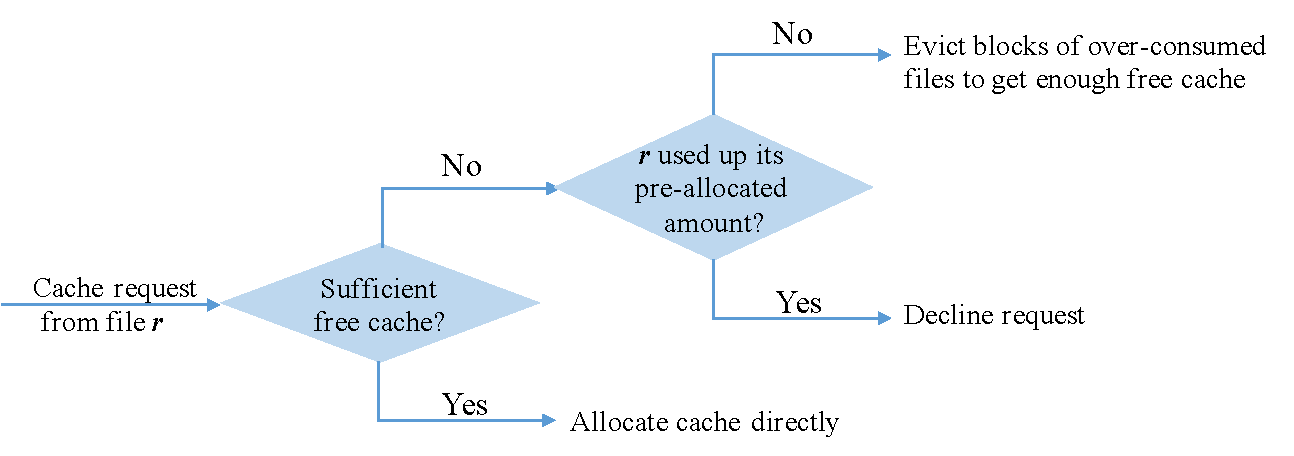
\includegraphics[scale=0.70]{figures-final/decision-making.pdf}
%	\caption{The decision-making process of EarnCache when a new cache space request occurs.}
%\end{figure}




\documentclass[10pt,conference,letterpaper]{IEEEtran}
\usepackage{graphicx}
\usepackage{subfigure}
\begin{document}
\section{experiment}

\begin{figure}[!htbp]
\centering
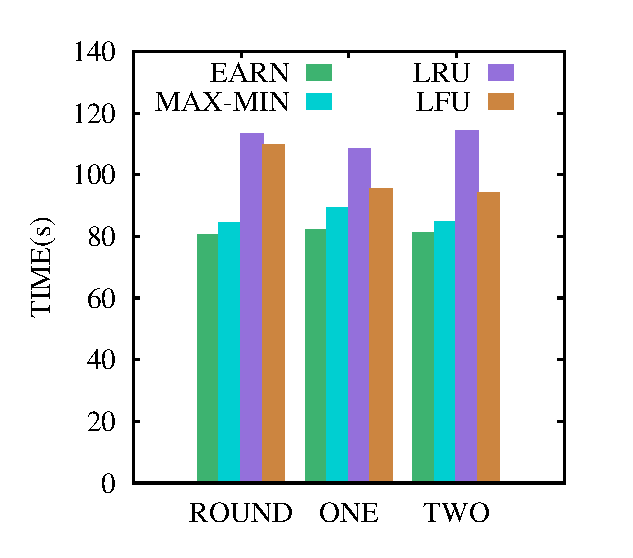
\includegraphics[scale=0.4]{figures/scan444_time.eps}
\caption{Access Time. Three files are equal in size (40GB).}
\label{fig:time_444}
\end{figure}

\begin{figure}[!htbp]
\centering
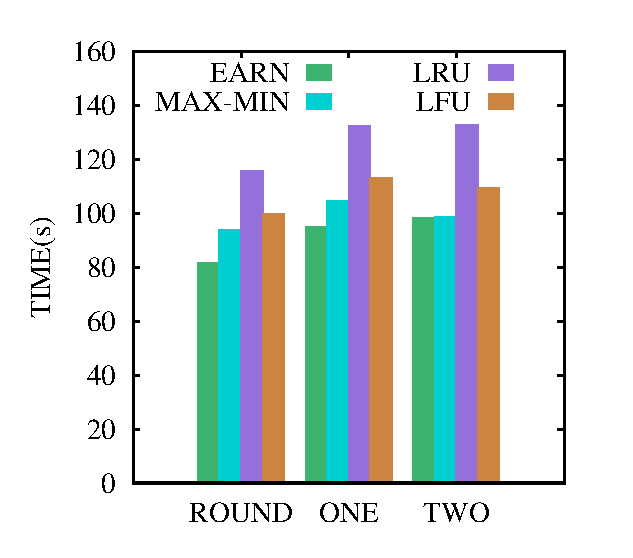
\includegraphics[scale=0.4]{figures/scan741_time.eps}
\caption{Access Time. The size of files is 70GB, 40GB and 10GB respectively.}
\label{fig:time_741}
\end{figure}

\begin{figure}[!htbp]
\centering
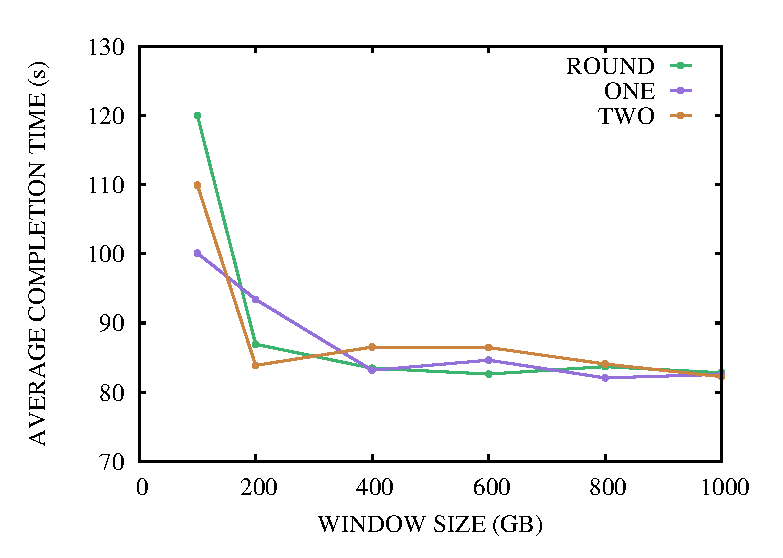
\includegraphics[scale=0.4]{figures/window_size_time.eps}
\caption{Access Time. Each with different window size.}
\label{fig:time_windowsize}
\end{figure}


\begin{figure}[!htbp]
    \subfigure[ROUND]{
    		\begin{minipage}[b]{0.25\linewidth}
    		\centering
    		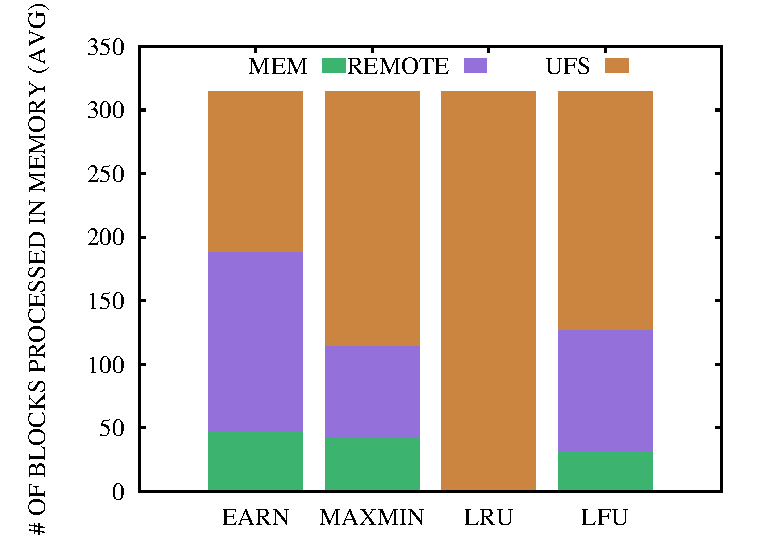
\includegraphics[scale=0.2]{figures/block_count_avg_round.eps}
    		\end{minipage}
    }
    \subfigure[ONE]{
        \begin{minipage}[b]{0.25\linewidth}
        \centering
        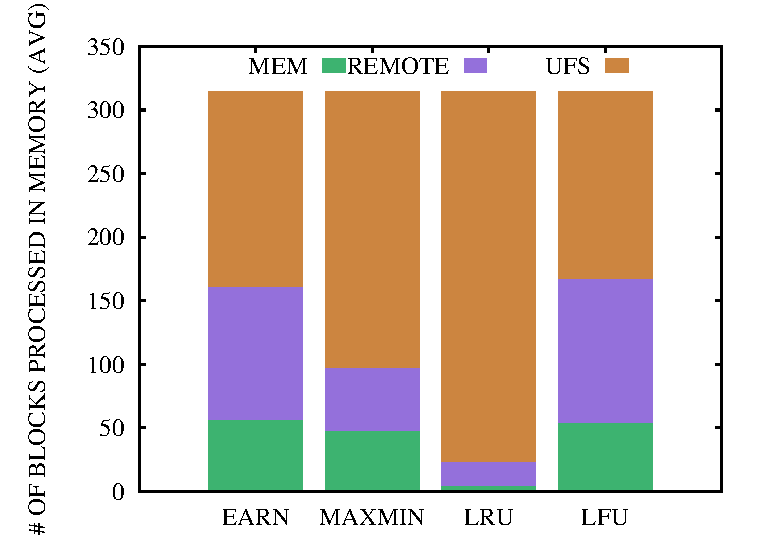
\includegraphics[scale=0.2]{figures/block_count_avg_one.eps}
        \end{minipage}
    }
    \subfigure[TWO]{
        \begin{minipage}[b]{0.25\linewidth}
        \centering
        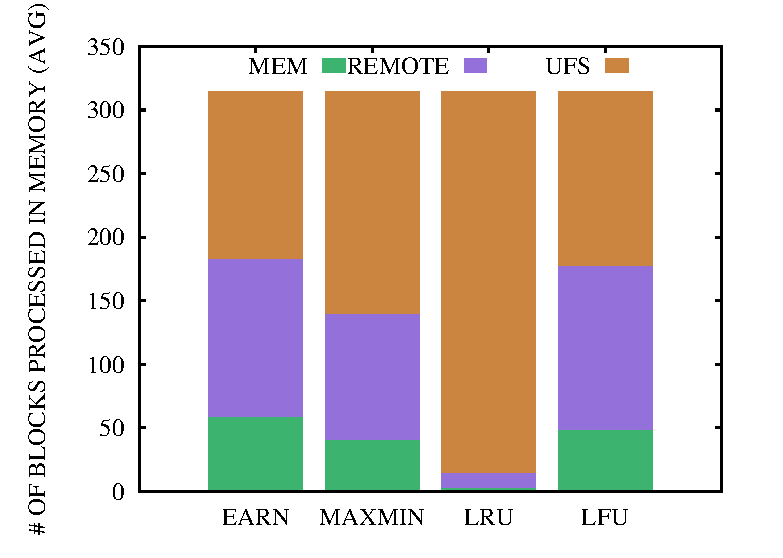
\includegraphics[scale=0.2]{figures/block_count_avg_two.eps}
        \end{minipage}
    }
    \caption{Distribution of blocks accessed in memory, remote memory and under file system.}
    \label{fig:block_count}
\end{figure}


\begin{figure}[!htbp]
    \subfigure[EARN]{
    		\begin{minipage}[b]{0.45\linewidth}
    		\centering
    		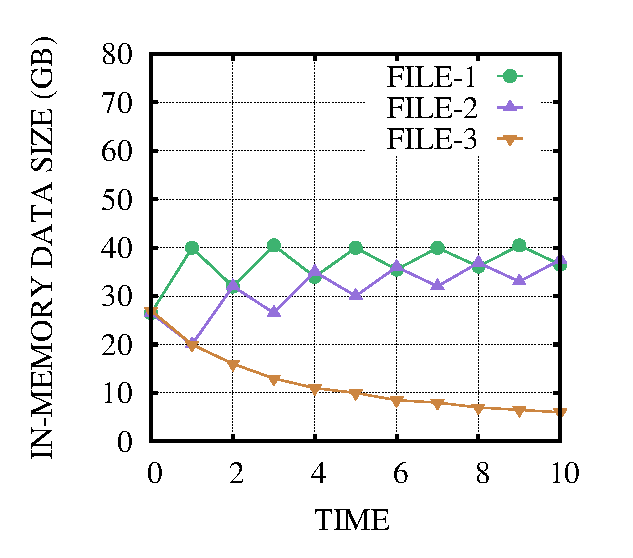
\includegraphics[scale=0.34]{figures/3-1-earn-1000-ds.eps}
    		\end{minipage}
    }
    \subfigure[MAXMIN]{
        \begin{minipage}[b]{0.45\linewidth}
        \centering
        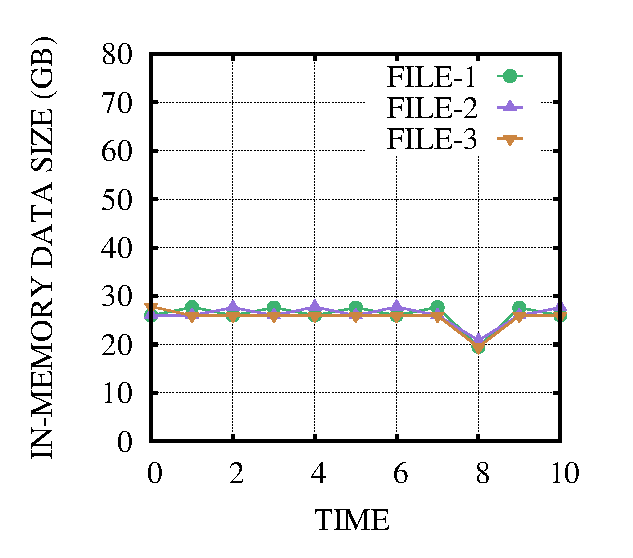
\includegraphics[scale=0.34]{figures/3-1-maxmin-1000-ds.eps}
        \end{minipage}
    }
    \caption{In-memory data size of each file after File-3 stops been visited.}
    \label{fig:3-1}
\end{figure}


\begin{figure}[!htbp]
    \subfigure[EARN]{
    		\begin{minipage}[b]{0.45\linewidth}
    		\centering
    		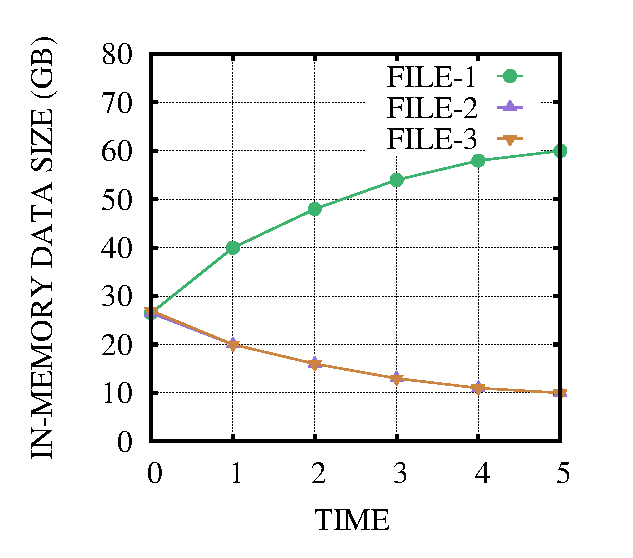
\includegraphics[scale=0.34]{figures/3-2-earn-1000-ds.eps}
    		\end{minipage}
    }
    \subfigure[MAXMIN]{
        \begin{minipage}[b]{0.45\linewidth}
        \centering
        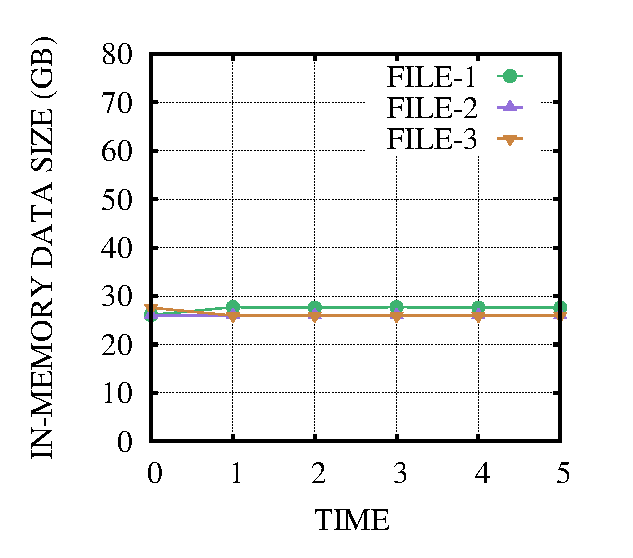
\includegraphics[scale=0.34]{figures/3-2-maxmin-1000-ds.eps}
        \end{minipage}
    }
    \caption{In-memory data size of each file after File-3 and File-2 stop been visited.}
    \label{fig:3-2}
\end{figure}

\end{document}

\documentclass[10pt,conference,letterpaper]{IEEEtran}
\usepackage{graphicx}

\usepackage{subfigure}
\begin{document}
\section{related work}
There has been various prior works on in-memory storage and caches. 
Cache for distributed storage systems is different from that in traditional single-node page-based file systems.
Simple cache replacement policies, like LRU, gain poor efficiency performance encountering big data scenarios.

Some framework-specific solutions include \cite{dist-cache-hdfs}, \cite{mapreduce-cache}, etc. 
\cite{mapreduce-cache} accelerates map-reduce process by caching temporary data between map and reduce processes.
HDCache~\cite{dist-cache-hdfs} is a distributed layered cache system built on the top of HDFS. It manages cache layer similarly to HDFS manages disk data, and organizes cache services in a P2P style using a distributed hash table.
On the other hand, our approach EARNCache along with Tachyon~\cite{tachyon} manages cache as a distributed file system, which can benefit a greater variety of computing frameworks and under file systems.

RAMCloud~\cite{ramcloud} proposes keeping information entirely in memory. Also various in-memory databases \cite{hstore} \cite{memcached} \cite{redis} store and process all data in memory. Spark~\cite{spark} also benefits from in-memory computing.
All-in-memory approach fits well in web services, while memory capacity becomes a bottleneck in big data semantics.

\cite{pacman}, \cite{fairride} and \cite{rate-aware} improve cache efficiency and fairness through different replacement strategies. 
PACMan~\cite{pacman} proposed LIFE and LFU-F policies. LIFE minimizes average completion time of jobs by favouring input files with smaller waves, and LFU-F maximizes cluster efficiency by favouring files that are accessed more frequently.
FairRide~\cite{fairride} focuses on management of shared resources and extends the max-min~\cite{maxmin}\cite{maxmin2} fairness with probabilistic blocking to avoid cheating.
\cite{rate-aware} proposed a dynamic partition strategy based on predicted utility on both fairness and performance. 
EARNCache also improves cache efficiency and fairness through new cache replacement policy. In comparison, EARNCache calculates base partition of memory by the access frequency information and adopts additional strategy to achieve fairness using the partition as a guide.



\begin{thebibliography}{1}

\bibitem{hadoop} http://hadoop.apache.org/

\bibitem{spark} http://spark.apache.org/

\bibitem{alluxio} http://www.alluxio.org/

\bibitem{memcached} https://memcached.org/

\bibitem{redis} http://redis.io/

\bibitem{dist-cache-hdfs} Zhang J, Wu G, Hu X, et al.
\newblock A distributed cache for hadoop distributed file system in real-time cloud services.
\newblock {\em International Conference on Grid Computing. IEEE.}, 2012: 12-21.

\bibitem{tachyon} Li H, Ghodsi A, Zaharia M, et al. 
\newblock Tachyon: Reliable, memory speed storage for cluster computing frameworks.
\newblock {\em SoCC.}, 2014.

\bibitem{rate-aware} Li Y, Feng D, Shi Z. 
\newblock Enhancing both fairness and performance using rate-aware dynamic storage cache partitioning.
\newblock  {\em International Workshop on Data-Intensive Scalable Computing Systems.} 2013.

\bibitem{pacman} Ananthanarayanan G, Ghodsi A, Wang A, et al. 
\newblock PACMan: coordinated memory caching for parallel jobs.
\newblock {\em NSDI.}, 2012.

\bibitem{fairride} Pu Q, Li H, Zaharia M, et al. 
\newblock FairRide: near-optimal, fair cache sharing.
\newblock {\em NSDI.} 2016. 

\bibitem{rdd} Zaharia M, Chowdhury M, Das T, et al. 
\newblock Resilient distributed datasets: A fault-tolerant abstraction for in-memory cluster computing.
\newblock {\em NSDI.} 2012.

\bibitem{mapreduce-cache} Zhang S, Han J, Liu Z, et al. 
\newblock Accelerating MapReduce with distributed memory cache.
\newblock {\em ICPADS.} 2009.

\bibitem{ramcloud} Ousterhout J, Agrawal P, Erickson D, et al. 
\newblock The case for RAMClouds: scalable high-performance storage entirely in DRAM. 
\newblock {\em ACM SIGOPS Operating Systems Review.} 2009.

\bibitem{hstore} Kallman R, Kimura H, Natkins J, et al. 
\newblock H-store: a high-performance, distributed main memory transaction processing system. 
\newblock {\em VLDB Endowment.} 2008.

\bibitem{maxmin} Ma Q, Steenkiste P, Zhang H.
\newblock Routing high-bandwidth traffic in max-min fair share networks
\newblock {\em SIGCOMM CCR.} 1996.

\bibitem{maxmin2} Cao Z, Zegura E W. 
\newblock Utility max-min: An application-oriented bandwidth allocation scheme
\newblock {\em INFOCOM.} 1999.


\end{thebibliography}


\end{document}

\section{Conclusion}\label{sec:Conclusion}

In this paper, we propose the EarnCache incremental big data caching mechanism for non-big clusters, which self-adaptively adjusts resource allocation strategies according to the competition condition of cache resources: evolving to incremental caching to depress competition when resources are in deficit, falling back to traditional on-demand-caching to expedite data caching-in when resources are in surplus. With EarnCache, files are not cached as a whole on demand, and applications or end users incrementally take over cache resources from others by accessing their datasets. EarnCache achieves improved resource utilization and performance.

%\bibliographystyle{abbrv}
%\bibliography{earn}

\begin{thebibliography}{99}%\scriptsize
%
\bibitem {dist-cache-hdfs}
J. Zhang, G. Wu, X. Hu, et al. A Distributed Cache for Hadoop Distributed File System in Real-Time Cloud Services. In Proceedings of GRID, 2012, pages 12-21.
%
\bibitem {ramcloud}
J. Ousterhout, P. Agrawal, D. Erickson, et al. The Case for RAMCloud. Communications of the ACM. Vol.54 No.7(2011), pages 121-130.

\bibitem {mapreduce}
J. Dean, S. Ghemawat, et al. MapReduce: Simplified data processing on large cluster. In Proceedings of OSDI, 2004, pages 137-150.%

\bibitem {tachyon}
H. Li, A. Ghodsi, M. Zaharia, et al. Tachyon: Reliable, Memory Speed Storage for Cluster Computing Frameworks. In Proceedings of SOCC, 2014, pages 6:1-6:15.
%
\bibitem {rate-aware}
Y. Li, D. Feng, Z. Shi. Enhancing Both Fairness and Performance Using Rate-aware Dynamic Storage Cache Partitioning. In Proceedings of DISCS, 2013, pages 31-36.
%
\bibitem{hdfs1}
K. Shvachko, H. Kuang, S. Radia, et al. The Hadoop Distributed File System. In Proceedings of MSST, 2010, pages 121-134.
%

\bibitem{pacman}
G. Ananthanarayanan, A. Ghodsi, A. Warfield, et al. PACMan: Coordinated Memory Caching for Parallel Jobs. In Proceedings of NSDI, 2012, pages 267-280.
%
\bibitem{fairride}
Q. Pu, H. Li, M. Zaharia, et al. FairRide: Near-Optimal, Fair Cache Sharing. In Proceedings of NSDI, 2016, pages 393-406.
%
\bibitem{rdd}
M. Zaharia, M. Chowdhury, T. Das, et al. Resilient Distributed Datasets: {A} Fault-Tolerant Abstraction for In-Memory Cluster Computing. In Proceedings of NSDI, 2012, pages 15-28.
%
\bibitem{mapreduce-cache}
S. Zhang, J. Han, Z. Liu, et al. Accelerating MapReduce with Distributed Memory Cache. In Proceedings of ICPADS, 2009, pages 472-478.
%

\bibitem{rcss}
Y. Luo, S. Luo, J. Guan, et al. A RAMCloud Storage System based on HDFS: Architecture, Implementation and Evaluation. Journal of Systems and Software. Vol.86 No.3(2013), pages 744-750.

\bibitem{maxmin}
Q. Ma, P. Steenkiste, H. Zhang. Routing High-Bandwidth Traffic in Max-Min Fair Share Networks. In Proceedings of SIGCOMM, 1996, pages 206-217.

\bibitem{maxmin2}
Z. Cao, W. Zegura. Utility Max-Min: An Application-Oriented Bandwidth Allocation Scheme. In Proceedings of INFOCOM, 1999, pages 793-801.

\bibitem{ltrf}
S. Tang, B. Lee, B. He, et al. Long-Term Resource Fairness: Towards Economic Fairness on Pay-as-you-use Computing Systems. In Proceedings of ICS, 2014, pages 251-260.

\bibitem{drf}
A. Ghodsi, M. Zaharia, B. Hindman, et al. Dominant Resource Fairness: Fair Allocation of Multiple Resource Types. In Proceedings of NSDI, 2011, pages 323-336.

%
\bibitem{redis}
Redis. http://redis.io.
%
\bibitem{hdfs2}
HDFS. http://hadoop.apache.org/hdfs.
%
\bibitem{hadoop} 
Hadoop. http://hadoop.apache.org.

\bibitem{spark} 
Spark. http://spark.apache.org.
%
\bibitem{memcached}
Memcached. http://danga.com/memcached.
\end{thebibliography}

\end{document}









